\documentclass{beamer}
\usepackage{graphicx}
\usepackage{tikz}
\usetikzlibrary{shapes,arrows}
\usepackage{tikz}
%\usecolortheme{seahorse}
  \setbeamertemplate{footline}[page number]

\setbeamertemplate{navigation symbols}{}
\setbeamertemplate{frametitle}[default][center]
\setbeamerfont{frametitle}{shape=\scshape}

\usepackage{xcolor}

\usepackage[flushleft]{threeparttable}

{\title{\textsc{Government Debt}}
\date{}
\author{Trevor Gallen}

\begin{document}
\renewcommand*{\inserttotalframenumber}{\pageref{lastframe}}

\begin{frame}
\titlepage
\end{frame}

\begin{frame}
\frametitle{Lecture 16.5 - Aside on Government Debt}
\begin{itemize}
\item Our discussion of trade \& the current account as savings gives a good jumping-off point to talk about government debt
\bigskip
\item Government debt plays a special role in economic events
\bigskip
\begin{itemize}
\item Frequently ubiquitously held within a country
\bigskip
\item Default can have far-ranging effects
\end{itemize}
\item Worth discussing on its own
\end{itemize}
\end{frame}


\begin{frame}
\frametitle{Definitions}
\begin{itemize}
\item The government's nominal budget constraint looks like:
$$\underbrace{\textcolor{red}{P_tG_t}+\textcolor{blue}{TR_t}+\textcolor{magenta}{R_{t-1}B_{t-1}^G}+\textcolor{orange}{B_{t-1}^G}}_{\text{Expenditure}}=\underbrace{\textcolor{gray}{T_t}+\textcolor{purple}{B_t^G}+M_t-M_{t-1}}_{Revenue}$$
Where:
\begin{itemize}
\item Nom govt spending: $\textcolor{red}{P_tG_t}$
\item Nom govt transfers: $\textcolor{blue}{TR_t}$
\item Nom govt interest payments: $\textcolor{magenta}{R_{t-1}B_{t-1}^G}$
\item Retiring govt bonds: $\textcolor{orange}{B_{t-1}^G}$
\item Nom tax revenue: $\textcolor{gray}{T_t}$
\item Nom new bonds issued: $\textcolor{purple}{B_t^G}$
\item Printed money: $M_t-M_{t-1}$
\end{itemize}
\item Could rewrite required deficit as:
$$Deficit=\textcolor{purple}{B_t^G}-\textcolor{orange}{B_{t-1}^G}=\textcolor{red}{P_tG_t}+\textcolor{blue}{TR_t}+\textcolor{magenta}{R_{t-1}B_{t-1}^G}-\textcolor{gray}{T_t}-\Delta M_t$$
\end{itemize}
\end{frame}

\begin{frame}
\frametitle{Definitions}
\begin{itemize}
\item Debt is a stock of money owed:  $B_{t-1}^G$
\bigskip
\item Deficit is the change in the stock of money owed: $\textcolor{purple}{B_t^G}-\textcolor{orange}{B_{t-1}^G}$
\bigskip
\item Let's look at some government debt over time
\bigskip
\item What's right measure?  Debt?  Deficit?  Debt/GDP?
\bigskip
\item Let's look at Debt/GDP first, equivalent to Debt/Income
\end{itemize}
\end{frame}

\begin{frame}
\frametitle{Definitions}
\begin{figure}
\centering
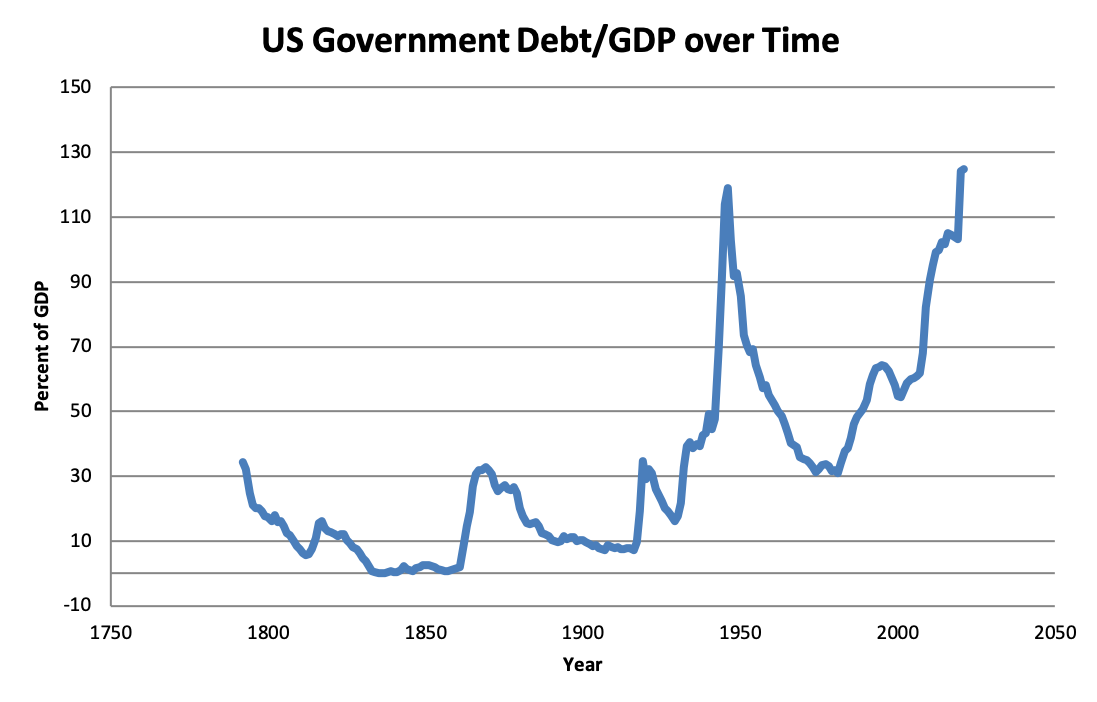
\includegraphics[scale=0.6]{Debt0.png}
\end{figure}
\end{frame}

\begin{frame}
\frametitle{Definitions}
\begin{figure}
\centering
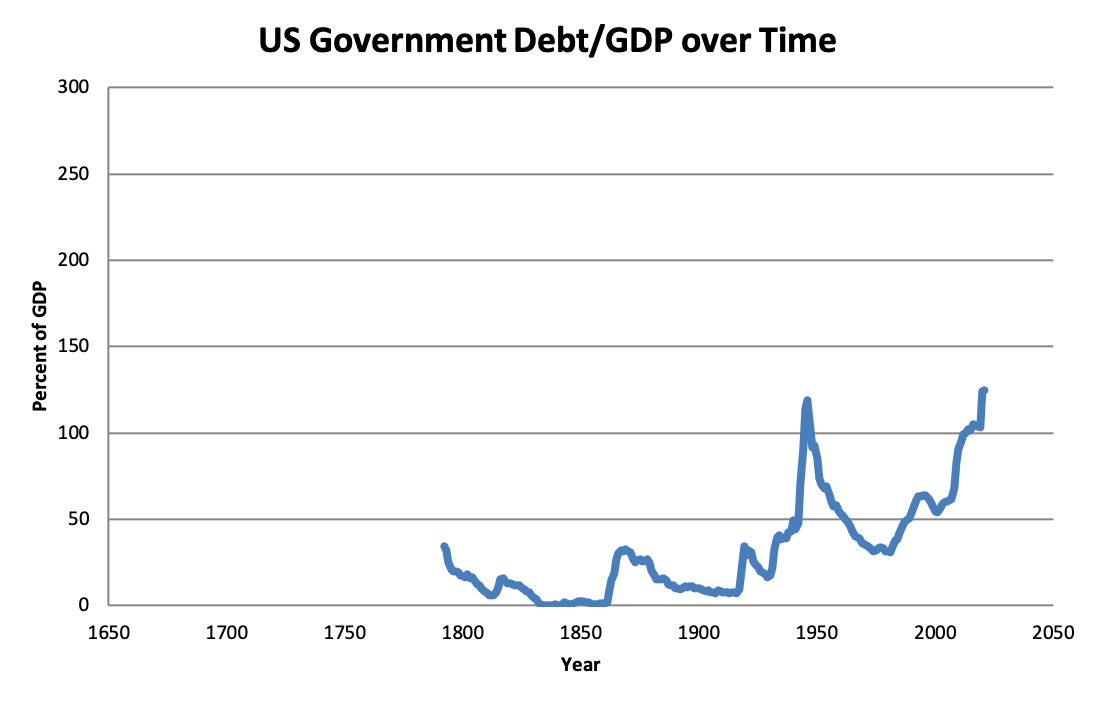
\includegraphics[scale=0.6]{Debt1.png}
\end{figure}
\end{frame}

\begin{frame}
\frametitle{Definitions}
\begin{figure}
\centering
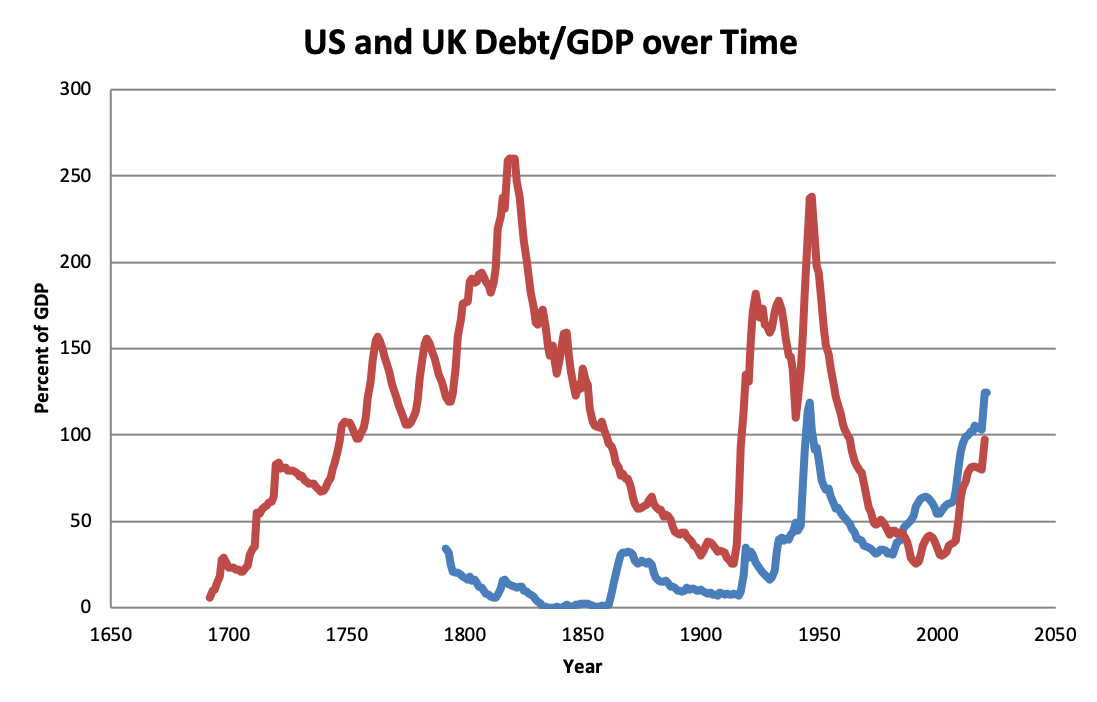
\includegraphics[scale=0.6]{Debt2.png}
\end{figure}
\end{frame}

\begin{frame}
\frametitle{Is the US Broke?}
\begin{itemize}
\item Note that debt owed by the US is in excess of 100\% of GDP
\bigskip
\item Does that mean it is ``broke?"
\bigskip
\item<2-> No!  I owe more than 100\% of my income to bank, but other things matter too
\bigskip
\item<3-> In our model, US government had no assets $A_t$ 
\bigskip
\item<4-> More importantly, what matters to not default is that:
$$\textcolor{gray}{T_t}+\Delta M_t+\textcolor{purple}{B_t^G}-\textcolor{orange}{B_{t-1}^G}-(\textcolor{red}{P_tG_t}+\textcolor{blue}{TR_t})\geq\textcolor{magenta}{R_{t-1}B_{t-1}^G}$$
\item<5-> For the whole path of $B_t^G$
\end{itemize}
\end{frame}

\begin{frame}
\frametitle{Intertemporal Budget Constraint}
\begin{itemize}
\item Could combine debt issuance to get:
$$\underbrace{\sum_{\tau=0}^\infty\frac{\textcolor{red}{P_{t+\tau}G_{t+\tau}}+\textcolor{blue}{TR_{t+\tau}}}{(1+R)^\tau}}_{\text{NPV expenditures}}=\underbrace{\sum_{\tau=0}^\infty \frac{\textcolor{gray}{T_{t+\tau}}+\Delta M_{t+\tau}}{(1+R)^\tau}}_{\text{NPV Income}}+\underbrace{B_t}_{\text{Initial Debt}}$$
\bigskip
\item Important: if RHS is growing faster than LHS, unlikely to be a problem
\bigskip
\item Easier to think of LHS as fraction of GDP $\tau Y_{t+\tau}$
\end{itemize}
\end{frame}


\begin{frame}
\frametitle{Sustainability}
\begin{itemize}
\item So, sustainability of debt does not mean that $B_t^G<Y_t$
\bigskip
\item It means that debt is not exploding as a fraction of GDP
\bigskip
\item What is maximum sustainable debt?
$$D^{max}=\tau\sum_{t=0}^\infty\left(\frac{1+g}{1+r}\right)^tY_0=\frac{1}{1-\frac{1+g}{1+r}}Y_0$$
\item So if $\tau=0.05$, $g=0.02$, $r=0.04$, $Y=1$, max debt \emph{without default }is 2.6x GDP
\item So if $\tau=0.05$, $g=0.01999$, $r=0.02$, $Y=1$, max debt \emph{without default }is 100,000x GDP
\item If $r\leq g$, maximum sustainable debt is infinite
\item Suggests that in current environments, debt isn't so costly
\end{itemize}
\end{frame}


\begin{frame}
\frametitle{Interest Rates and Growth Rates}
\begin{figure}
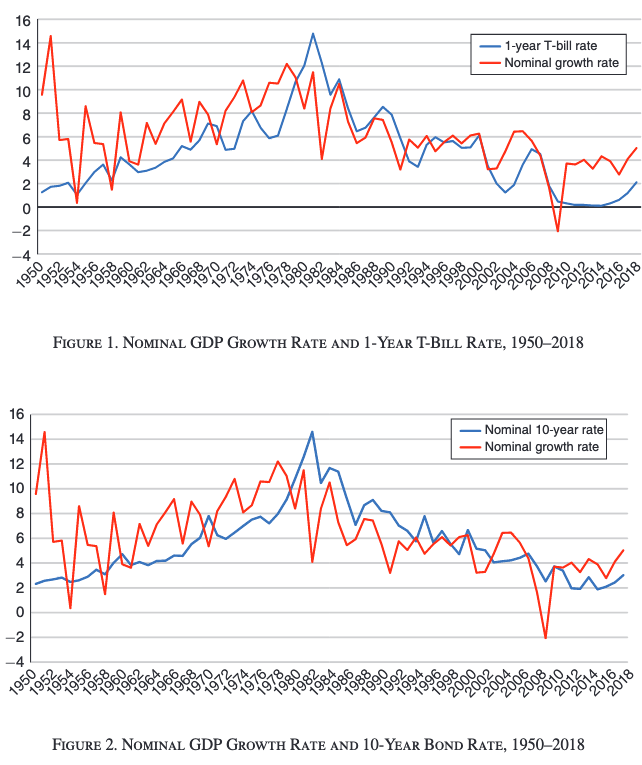
\includegraphics[scale=0.3]{Blanchard1.png}
\end{figure}
\end{frame}


\begin{frame}
\frametitle{Blanchard}
\begin{itemize}
\item $$d_t=\frac{1+r}{1+g}d_{t-1}+x_t$$
\item Where $d_t$ is debt/gdp, $r$ is interest rate, $g$ is growth rate of GDP, and $x$ is (non-interest expenditures)-income (primary deficit)
\bigskip
\item Let's say we pay for programs but borrow to pay interest, so $x$ is zero
\end{itemize}
\end{frame}


\begin{frame}
\frametitle{Debt under zero primary deficit}
\begin{figure}
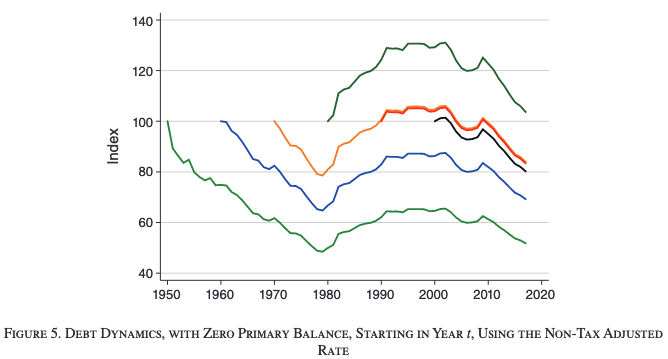
\includegraphics[scale=0.5]{Blanchard2.png}
\end{figure}
\end{frame}

\begin{frame}
\frametitle{Public Debt}
\begin{itemize}
\item When $r$ is small, public debt is cheap
\bigskip
\item But sometimes that leads to disaster:  sovereign default  (implicit or explicit)
\bigskip
\item Let's visit more
\end{itemize}
\end{frame}

\begin{frame}
\frametitle{Issues in Measurement}
\begin{itemize}
\item Who owns debt matters
\bigskip
\begin{itemize}
\item ``External" debt held by foreigners
\bigskip
\item ``Internal" debt held domestically
\bigskip
\item Within ``internal," government vs. public
\end{itemize}
\bigskip
\item 50\% of debt held by private domestic investors
\bigskip
\item 24\% held domestically by government
\bigskip
\item 26\% held by foreign investors  
\begin{itemize}
\item 4.6\% by Japan
\bigskip
\item 3.8\% by Mainland China
\bigskip
\item 1.6\% by UK
\end{itemize}
\end{itemize}
\end{frame}

\begin{frame}
\frametitle{When countries can't pay, what happens?}
\begin{itemize}
\item Sometimes countries can't (or won't) pay
\bigskip
\item What happens?
\begin{itemize}
\item Inflation (or debasement, currency crash)
\begin{itemize}
\item If need nominal currency, can always pay
\item If need real currency, inflation is one method
\end{itemize}
\bigskip
\item External debt default: no longer pay debt obligations to foreigners (typically in another country's currency)
\bigskip
\item Internal debt default: no longer pay debt obligations to domestic holders (typically in own currency)
\end{itemize}
\end{itemize}
\end{frame}

\begin{frame}
\frametitle{Defaults are not uncommon}
\begin{figure}
\centering
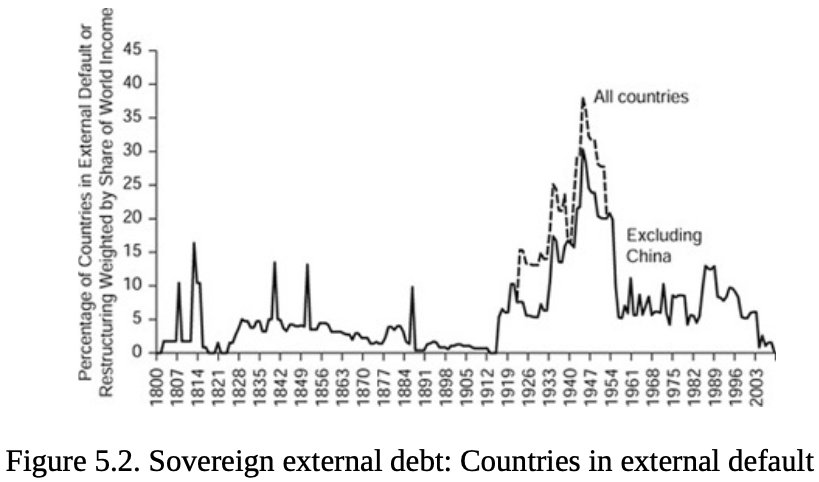
\includegraphics[scale=0.4]{RR1.png}
\end{figure}
\end{frame}

\begin{frame}
\frametitle{Defaults are not uncommon}
\begin{figure}
\centering
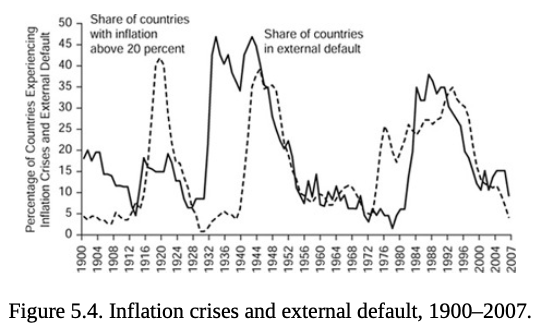
\includegraphics[scale=0.5]{RR2.png}
\end{figure}
\end{frame}

\begin{frame}
\frametitle{Serial Defaulting}
\begin{itemize}
\item ``Debt intolerance is a syndrome in which weak institutional structures and a problematic political system make external borrowing a tempting device for
governments to employ to avoid hard decisions about spending and taxing."
\bigskip
\item Idea is that the political structure of some countries makes defaulting under low debt thresholds ``desirable"
\begin{table}
\begin{tabular}{ll}
\multicolumn{2}{c}{External Debt at the Time of Default: 1970-2008}\\
\hline\hline
Range of External Debt/GDP & Percent of total defaults\\
\hline
$<$40\% & 19.4\% \\
41-60\% & 32.3\% \\
61-80\% & 16.1\% \\
81-100\% & 16.1\% \\
$>$100\% & 16.1\% \\
\hline\hline
\end{tabular}
\end{table} 
\end{itemize}
\end{frame}

\begin{frame}
\frametitle{Serial Defaulting}
\begin{figure}
\centering
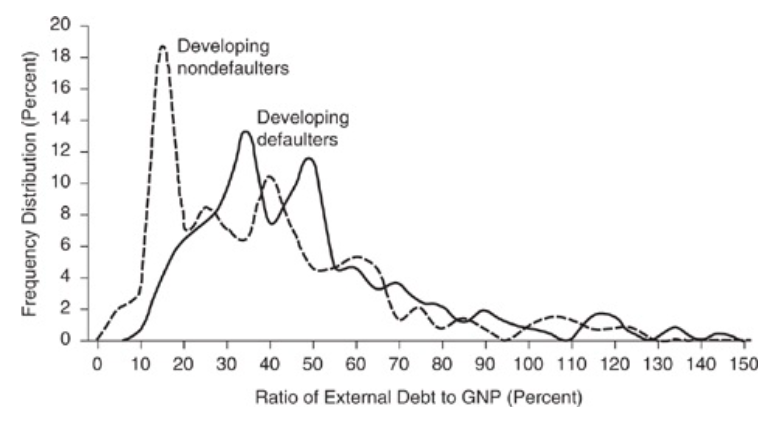
\includegraphics[scale=0.4]{RR3.png}
\end{figure}
\end{frame}


\begin{frame}
\frametitle{Issues with Foreign Debt-I }
\begin{itemize}
\item Russian revolution in 1918 repudiated 16 billion rubles in foreign debt
\bigskip
\item For the next 80 years, debtholders and their descendants fought to get paid
\bigskip
\item Czarist assets frozen (eventually used to pay creditors)
\bigskip
\item Could not raise money on public markets throughout its existence (governmental and private loans occurred)
\bigskip
\item Eventually settled in 1996
\end{itemize}
\end{frame}


\begin{frame}
\frametitle{Issues with Foreign Debt-II }
\begin{itemize}
\item In 2001 Argentina defaulted on debt issued in US 
\bigskip
\item Paid roughly \$0.27 on the dollar (very steep)
\bigskip
\item In 2005, 76\% agreed, but 24\% were holdouts
\bigskip
\item Reopened in 2010 and got down to 8\% holdouts
\bigskip
\item Holdout creditors great nusiance
\end{itemize}
\end{frame}

\begin{frame}
\frametitle{Issues with Foreign Debt-II}
\begin{figure}
\centering
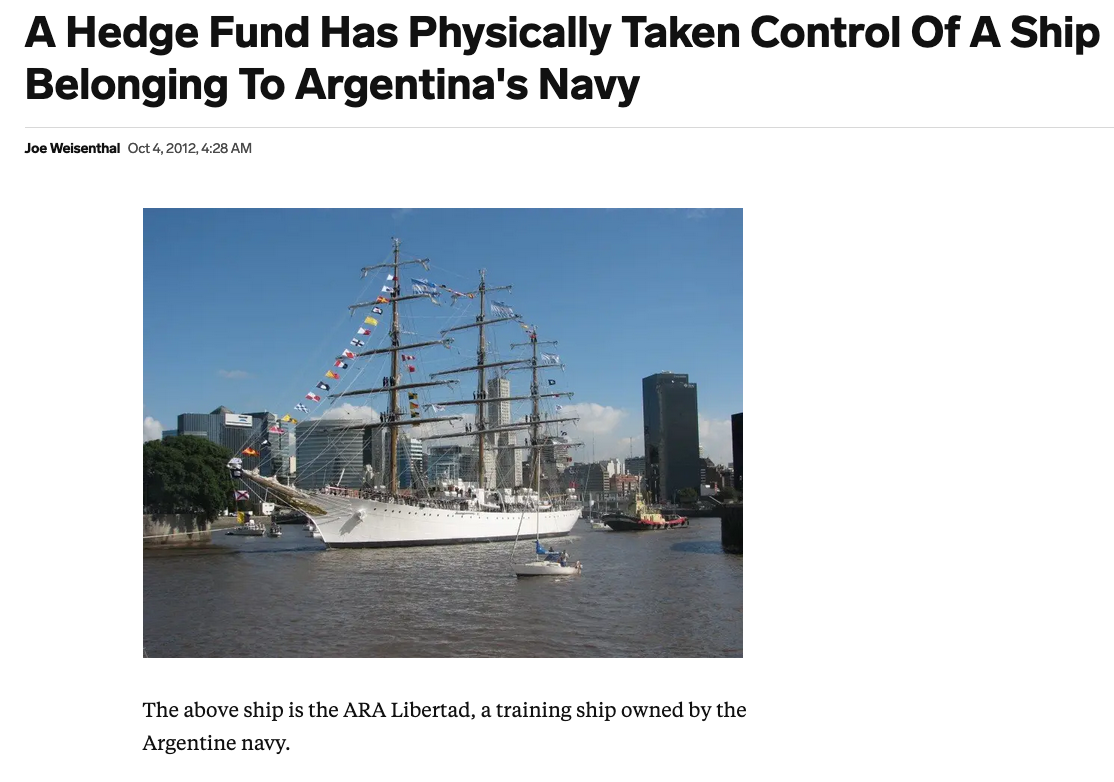
\includegraphics[scale=0.3]{Liberdad.png}
\end{figure}
\end{frame}

\begin{frame}
\frametitle{Issues with Foreign Debt-II }
\begin{itemize}
\item Eventually it was decided that holdouts had strong legal standing, because Argentina deliberately gave up sovereignty
\bigskip
\item Holdouts by and large paid in full
\bigskip
\item Reopened in 2010 and got down to 8\% holdouts
\bigskip
\item Holdout creditors great nuisance
\bigskip
\item Couldn't pay holdouts full amount (RUFO)
\bigskip
\item Couldn't not pay holdouts (pari passu)
\bigskip
\item Eventually resolved circa 2016
\end{itemize}
\end{frame}

\begin{frame}
\frametitle{Are ``vulture" funds bad?}
\begin{itemize}
\item Con: gum up the works, lock out Argentina for 5-10 extra years, slow growth
\bigskip
\item Pro: Raises cost of default ex-ante (deters)
\bigskip
\item Con:  Raises cost of default ex-post (``no point" in punishing ex-post (except future ex-ante!))
\bigskip
\item Pro: Partially resolves coordination issues for ``the little guy"
\end{itemize}
\end{frame}

\begin{frame}
\frametitle{Issues with Foreign Debt-III }
\begin{itemize}
\item From 1832-1949, Newfoundland independent (circa fifth-oldest parliament)
\bigskip
\item Went into debt $>$300\% of GDP, deficits of 10\% of GDP
\bigskip
\item Pressured by UK and Canada to be absorbed by Canada
\bigskip
\item Syncs with gunboat diplomacy
\end{itemize}
\end{frame}

\begin{frame}
\frametitle{Costs of Foreign debt }
\begin{itemize}
\item Some papers attempt to estimate the costs of foreign default
\bigskip
\item Let's look at a few
\end{itemize}
\end{frame}

\begin{frame}
\frametitle{Cruces and Trebesch  2013 }
\begin{figure}
\centering
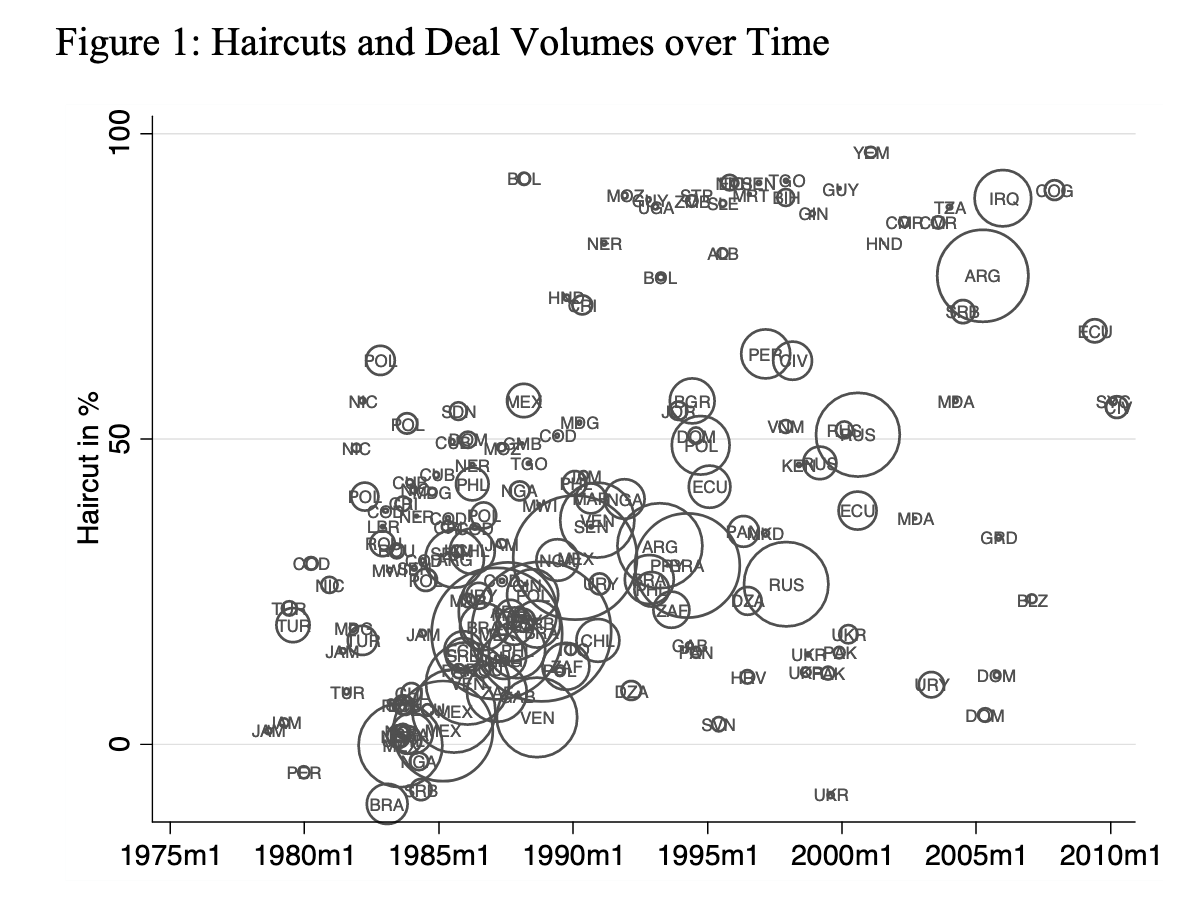
\includegraphics[scale=0.5]{CrucesTrebesch.png}
\end{figure}
\end{frame}

\begin{frame}
\frametitle{Cruces and Trebesch  2013 }
\begin{figure}
\centering
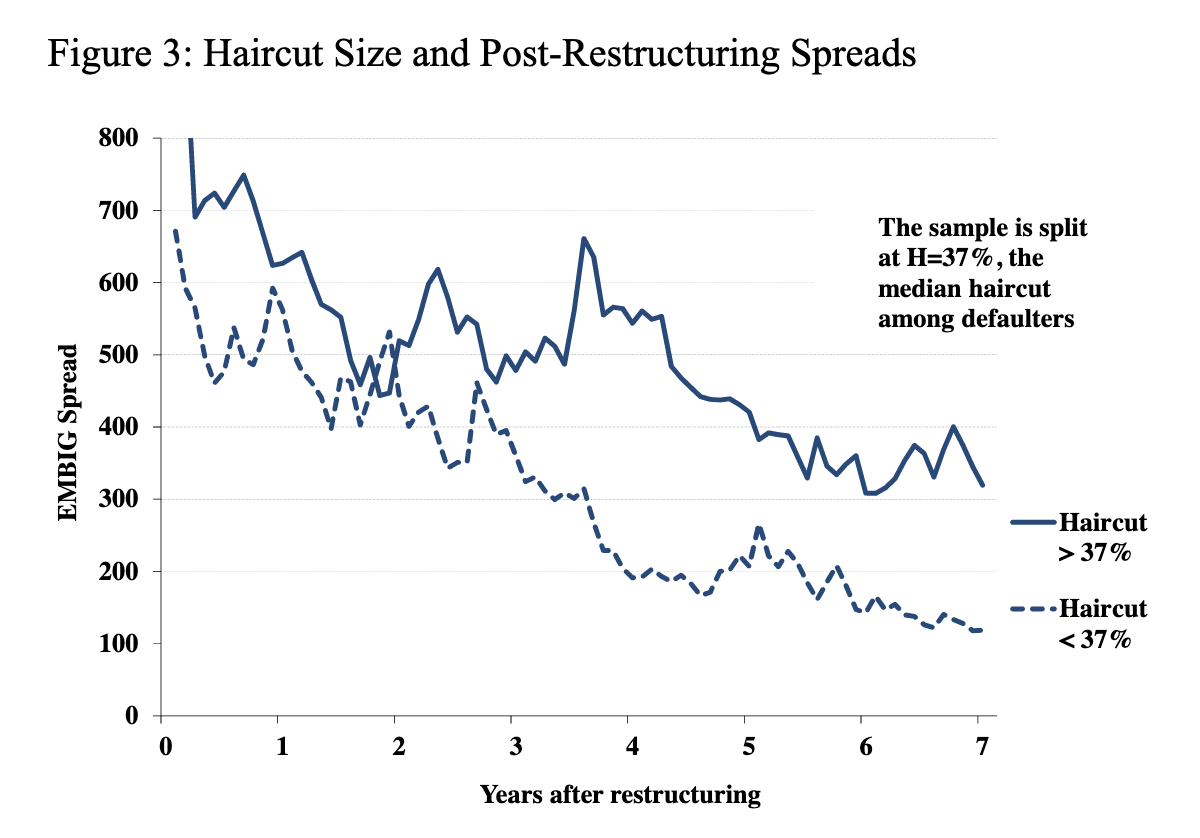
\includegraphics[scale=0.5]{CrucesTrebesch2.png}
\end{figure}
\end{frame}


\begin{frame}
\frametitle{Andrade and Chhaochharia 2017 }
\begin{itemize}
\item Some stock prices are sensitive to sovereign default risk
\bigskip
\item In Greek default, 97\% of bondholders accepted a 60\% haircut on claims(!)
\bigskip
\item Idea:  look at firms that have low asset tangibility, and high bank dependence or bank dependence on PIIGS
\bigskip
\item Find that such firms (which make up $\sim$70\% of assets are very vulnerable to default (act as if default would destroy 12\% of productive assets(!)) 
\bigskip
\item Similar, but for Argentina: 
\begin{itemize}
\item Exposure to Argentine default suggests big losses to firm values (1\% increase in default, equity values drop by 0.55\%!)
\end{itemize}
\end{itemize}
\end{frame}

\begin{frame}
\frametitle{Andrade and Chhaochharia 2017 }
\begin{figure}
\centering
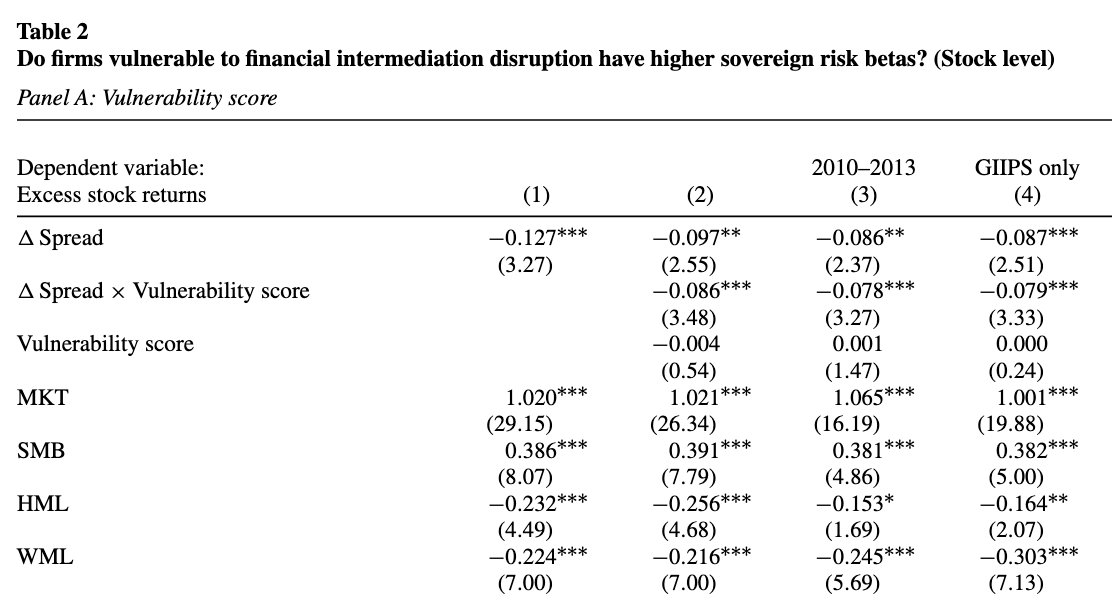
\includegraphics[scale=0.6]{AndradeChhaochharia1.png}
\end{figure}
\end{frame}

\begin{frame}
\frametitle{Kuvshinov and  Zimmermann 2019}
\begin{itemize}
\item Try to compare like countries based on probability of default but some defaulted
\bigskip
\item Let's look at their results
\end{itemize}
\end{frame}

\begin{frame}
\frametitle{Kuvshinov and  Zimmermann 2019}
\begin{figure}
\centering
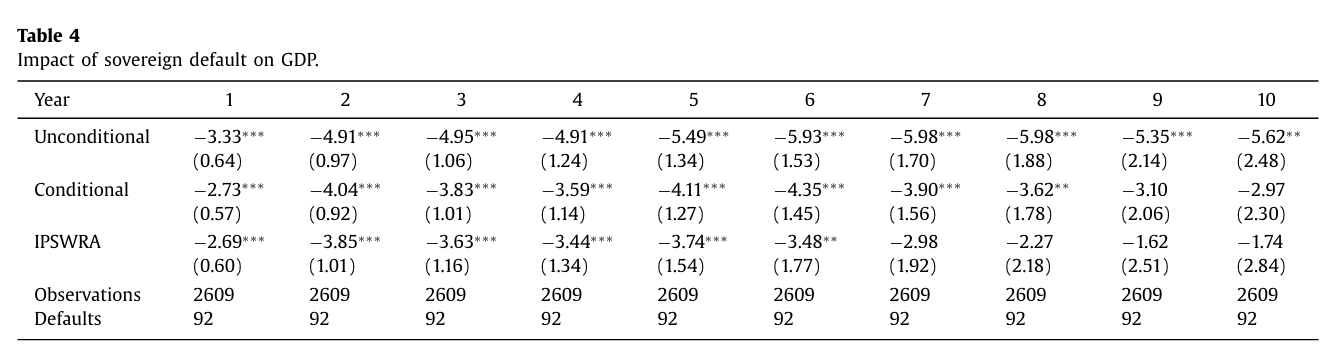
\includegraphics[scale=0.6]{Kuvshinov_1.png}
\end{figure}
Controls matter! (Hard problem)
\end{frame}

\begin{frame}
\frametitle{Kuvshinov and  Zimmermann 2019}
\begin{figure}
\centering
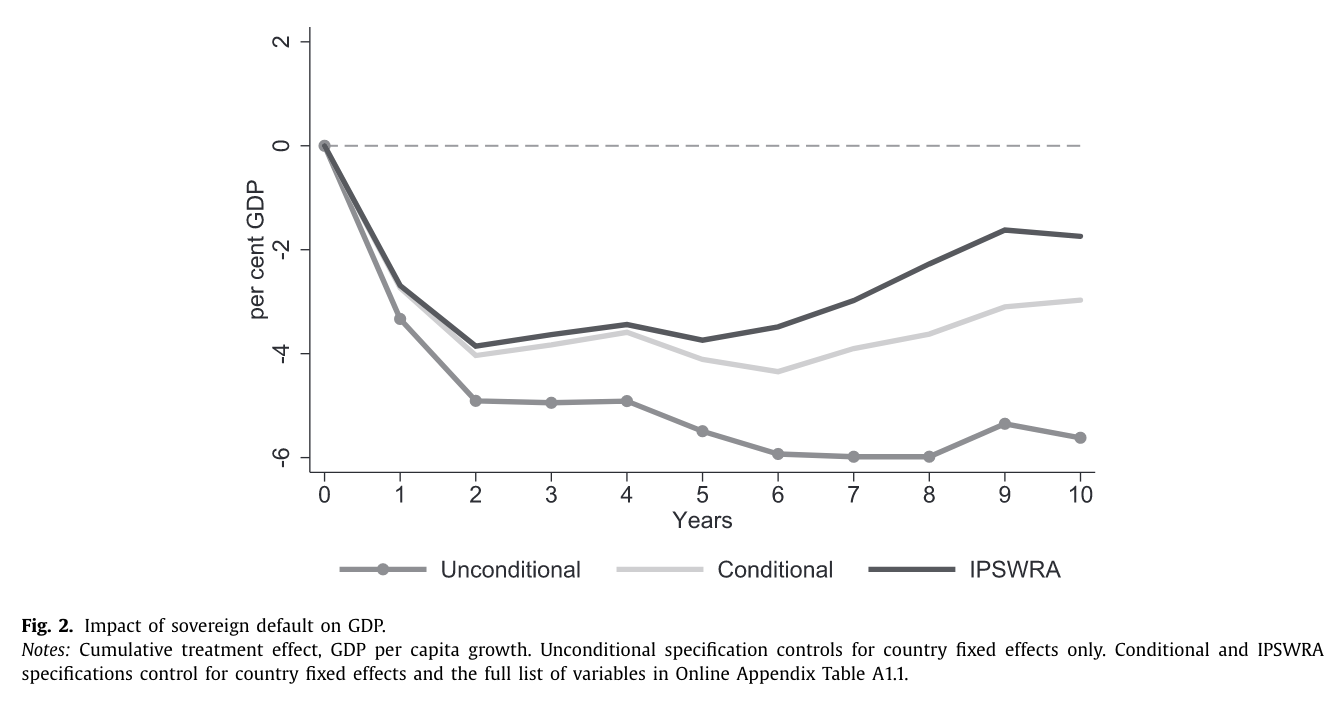
\includegraphics[scale=0.5]{Kuvshinov_2.png}
\end{figure}
While effects level off, loss of $\approx$33\% of GDP over the course of 10 years!
\end{frame}

\begin{frame}
\frametitle{Kuvshinov and  Zimmermann 2019}
\begin{figure}
\centering
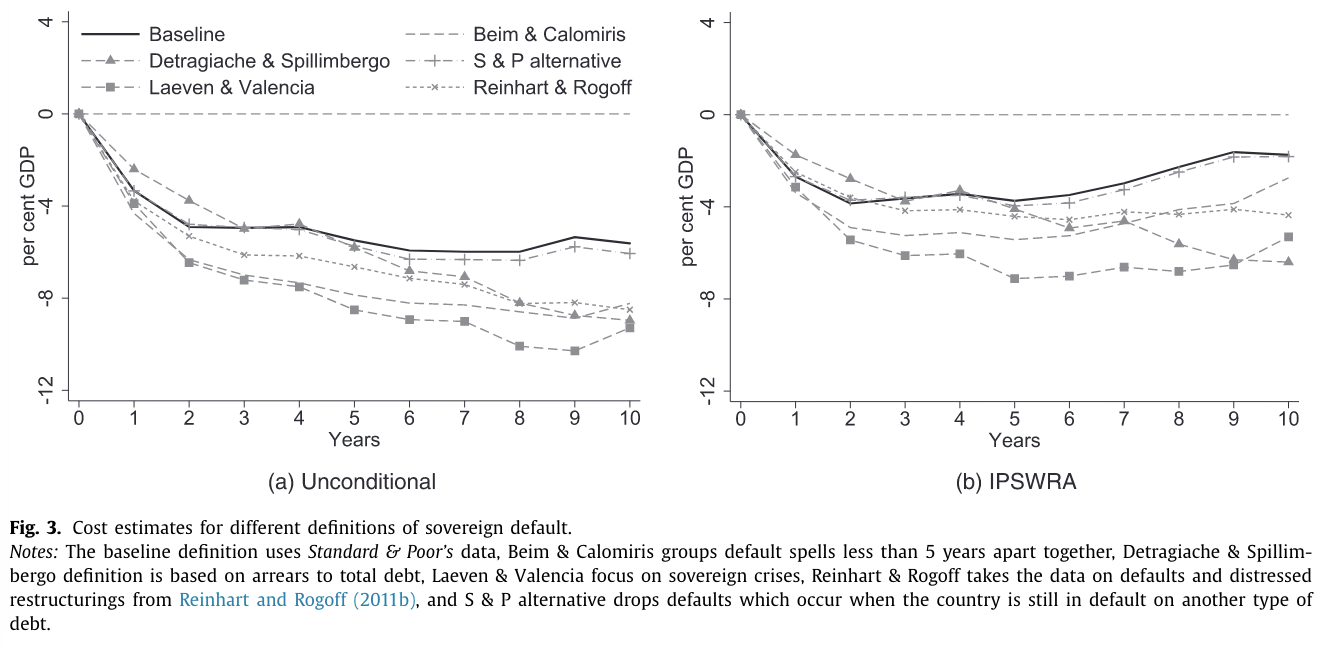
\includegraphics[scale=0.5]{Kuvshinov_3.png}
\end{figure}
Many different ways of trying to solve
\end{frame}


\begin{frame}
\frametitle{Kuvshinov and  Zimmermann 2019}
\begin{figure}
\centering
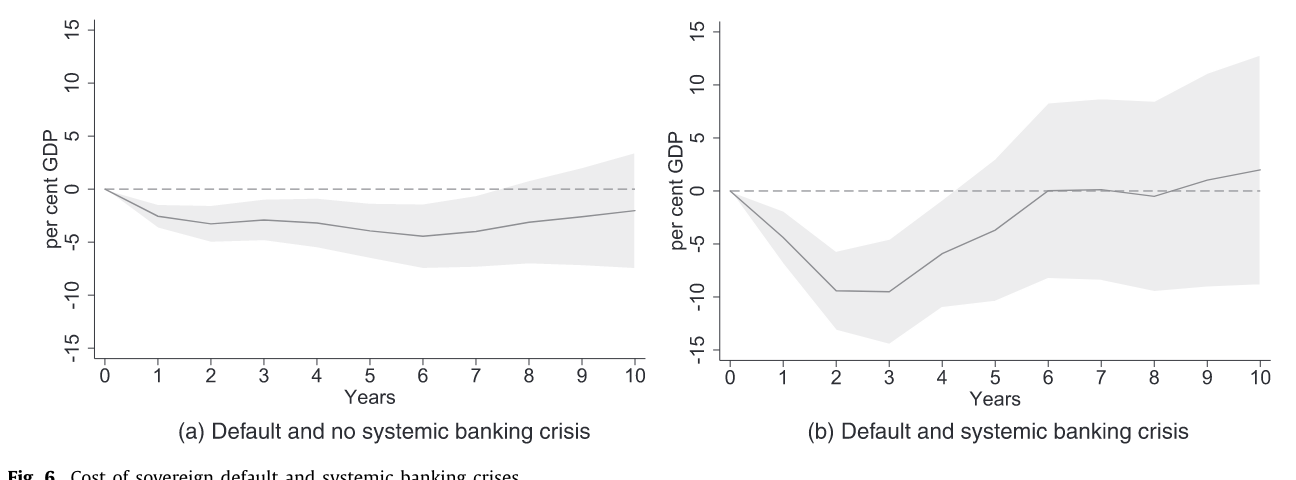
\includegraphics[scale=0.5]{Kuvshinov_4.png}
\end{figure}
Enormous heterogeneity in response depending on banking crisis
\end{frame}

\begin{frame}
\frametitle{Kuvshinov and  Zimmermann 2019}
\begin{figure}
\centering
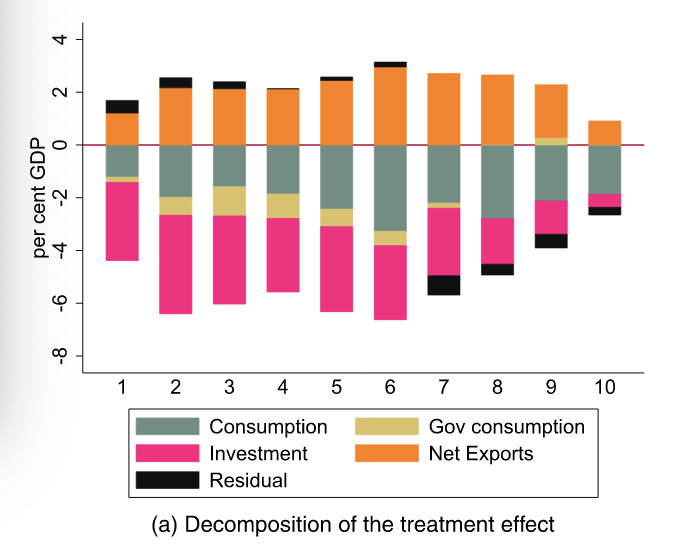
\includegraphics[scale=0.7]{Kuvshinov_5.png}
\end{figure}
Effect on exports positive, but domestic effects outweigh
\end{frame}


\begin{frame}
\frametitle{Kuvshinov and  Zimmermann 2019}
\begin{figure}
\centering
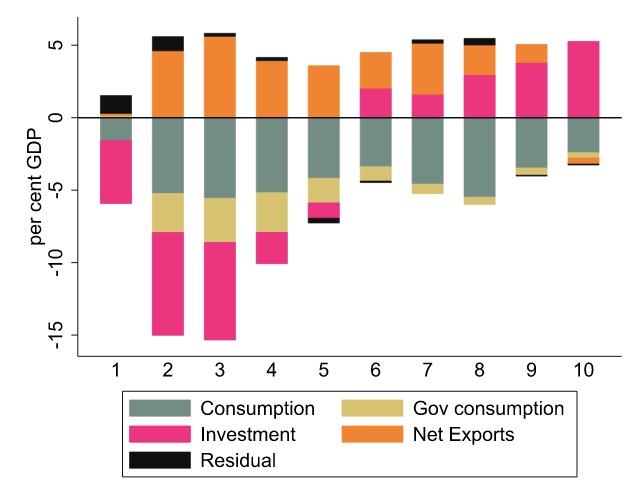
\includegraphics[scale=0.7]{Kuvshinov_6.png}
\end{figure}
Same, but for sovereign banking crisis.  Kill investment and consumption
\end{frame}

\begin{frame}
\frametitle{Cruces Zabel 2017 }
\begin{figure}
\centering
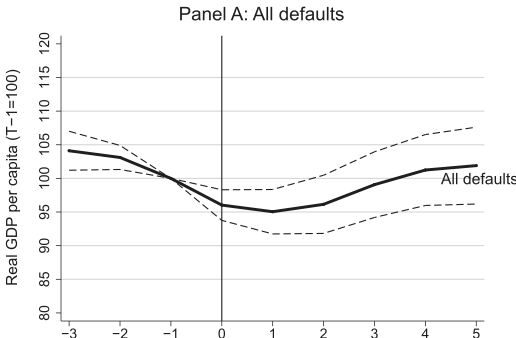
\includegraphics[scale=1]{Cruces1.png}
\end{figure}
\end{frame}

\begin{frame}
\frametitle{Cruces Zabel 2017 }
\begin{figure}
\centering
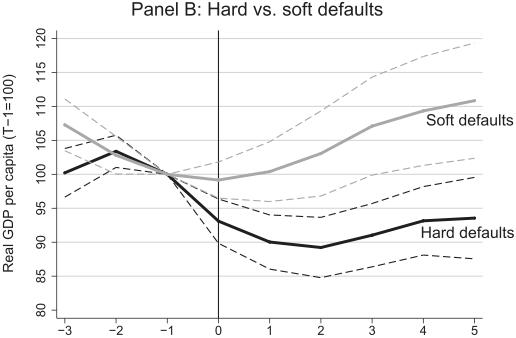
\includegraphics[scale=1]{Cruces2.png}
\end{figure}
\end{frame}


\begin{frame}
\frametitle{Thoughts}
\begin{itemize}
\item Government debt is potentially useful!
\bigskip
\item If your government is responsible, tool for good, not burdensome in current regime
\bigskip
\item But governments default all the time
\bigskip
\item The economic costs of default are not small, and the political consequences are even larger
\bigskip
\item There are no free lunches: the worse the default, the worse the consequences
\bigskip
\item Using vs playing with fire
\end{itemize}
\end{frame}


%\begin{frame}
%\frametitle{Option 1: Inflation}
%\begin{itemize}
%\item Pro:  is ``soft," in that most debt is nominal, not likely to cause banking crises
%\bigskip
%\item Pro: unlikely to lock you out of trade entirely
%\bigskip
%\item Con: if pensioners hold nominal debt, you crush them
%\bigskip
%\item Con: as a financial friction, reduces real GDP
%\bigskip
%\item Con: ease of default makes default more likely
%\end{itemize}
%\end{frame}
%
%\begin{frame}
%\frametitle{Option 1: External Default}
%\begin{itemize}
%\item Pro:  is ``soft," in that most debt is nominal, not likely to cause banking crises
%\bigskip
%\item Pro: unlikely to lock you out of trade entirely
%\bigskip
%\item Con: if pensioners hold nominal debt, you crush them
%\bigskip
%\item Con: as a financial friction, reduces real GDP
%\bigskip
%\item Con: ease of default makes default more likely
%\end{itemize}
%\end{frame}



\end{document}